%!TEX root = ../../master.tex
\section{Software}
The previous sections described the process of designing and building a physical cluster. We now turn the focus to the decisions made regarding software in building KubeCloud. The involved layers will be described and discussed from the operating system layer to the application layer.


\subsection*{Operating System}
Hypervisors are often used in data centers (Chapter~\ref{chap:fundamentals_cloud}) and could be an interesting topic to investigate. The limited resources on a Raspberry Pi, however, does not allow for powerful enough partitions of the resources into virtual machines. Furthermore, the partitioning contradicts the purpose of the physical representation of the concepts in cloud computing. KubeCloud is, therefore, a bare-metal cluster without virtual machines. \\

\noindent
The choice of operating system (OS) is important since the rest of the software need to run on top of it. Stability is one of the most important properties of the OS for KubeCloud.
A Linux distribution is needed to run Docker and Kubernetes. We did not have a particular distribution preference but looking at the available options in the ARM community led to the choices of HypriotOS, Raspbian, or Arch Linux. The intention was to build on top of already configured distributions to keep the focus on the usage of the cluster.

\subsubsection*{The Road to a Stable OS}
Several different configurations of operating systems combined with different Docker and Kubernetes versions have been tried out on the road to stability to address the requirement \textit{"KubeCloud shall allow for shutdown and restart with a frequency twice a week"}. \\

\noindent
\textit{HypriotOS with k8s-on-rpi} \\
At first, HypriotOS\footnote{\url{http://blog.hypriot.com/downloads/}}(v0.6.1) was tried out. HypriotOS is an extension of the default Raspberry Pi OS (Raspbian).  Installation of HypriotOS is easy, and it has Docker installed out of the box. HypriotOS seemed like a good solution since Kubernetes was easy to get up and running on the clusters using k8s-on-rpi\footnote{\url{https://github.com/awassink/k8s-on-rpi}}. Unfortunately, stability issues arose after restarting the clusters, which became evident when Kubernetes became unresponsive. The time used for scheduling of pods experienced an increase and failed in many cases. \\


\noindent
\textit{HypriotOS with kubernetes-on-arm} \\
Another Kubernetes project called kubernetes-on-arm\footnote{\url{https://github.com/luxas/kubernetes-on-arm}} was installed on top of HypriotOS (v0.6.1), but the stability issues were still present. The debugging was time-consuming since we had to flash SD cards, assign static IPs, install Kubernetes, and wait for the errors to appear. \\


\noindent
\textit{ArchLinux with kubernetes-on-arm} \\
Since the common factor in the two previous configurations was the operating system, a new operating system was investigated. An ArchLinux installation from the kubernetes-on-arm project turned out to (almost) be the end of the road of our stability issues. In order to automate and adjust the project to our setup, scripts were created for automation purposes. These scripts are described in further detail in the upcoming section on Kubernetes. \\


%% Docker
\subsection*{Docker}
As described in Section~\ref{sec:role_of_os_and_hypervisors}, containers such as Docker have gained much attention the last couple of years because of the benefits they provide. Figure~\ref{fig:flow_spring_software} shows Docker's role in the cluster. Applications (Spring Boot) are containerized into a Docker image with the needed dependencies. The Kubernetes infrastructure is using the Docker images to manage the cluster.
\begin{figure}[H]
    \centering
    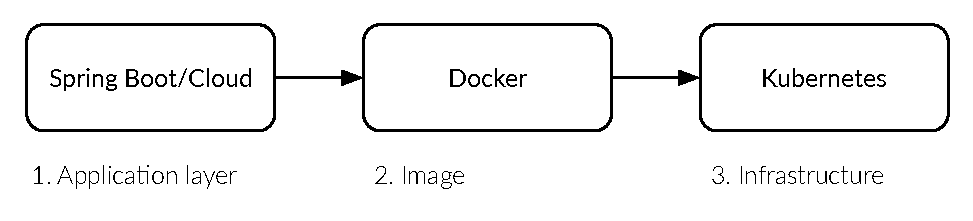
\includegraphics[width=12cm]{figures/flow_overview}
    \caption{Flow Overview}
    \label{fig:flow_spring_software}
\end{figure}

\noindent
Installing Docker on a Raspberry Pi is not difficult, but since the Raspberry Pi runs on ARM architecture, all Docker images must be built for ARM. Most developer machines do not use ARM, and cross-compilation or building on an ARM device is, therefore, necessary. One of the ideas behind Docker is that applications and dependencies can be packaged together and recreated in the production environment. The ARM architecture limitation is unfortunate, but it has not been a big problem. Two very similar base images of Java 8 have been used for the ARM and amd64 architectures to accommodate this challenge.

\noindent The previously described ArchLinux configuration comes with the installation of Docker used in KubeCloud.
%% /Docker

\subsection*{Kubernetes}
Kubernetes (v1.2) was chosen as cluster management system for several reasons. The previously mentioned transformation from being machine-oriented to application-oriented combined with the increased tendency of containerization led to the decision of using containers and Kubernetes. Furthermore, containers are more lightweight than virtual machines, and since the Raspberry Pi has restricted resources compared to a server it seemed like a good idea to reduce the overhead. In order to illustrate concepts of resilience, Kubernetes offers several interesting approaches to adaptive capacity (Figure~\ref{fig:our_resilience_definition}) on the infrastructure level resilience. Among those are replication, heartbeats, and automatic rescheduling when pods fail, which leads to rapidity. Many of Kubernetes' concepts can be used to illustrate resilience on a physical cluster. \\

\noindent
Kubernetes is used to manage Docker containers on the Raspberry Pis in KubeCloud. Each Raspberry Pi node is registered as a node in the cluster and is thereby a small-scale bare-metal server running Kubernetes. On managed solutions such as Google Container Engine, a virtual machine is used per node instead of a Raspberry Pi. In KubeCloud, Kubernetes schedules workloads (containers) across the different Raspberry Pis (nodes). \\

\noindent
As previously described, the road to stability led to a configuration with ArchLinux and the kubernetes-on-arm project. Kubernetes-on-arm furthermore comes with many features such as a command-line tool to enable masters and workers and to manage add-ons. One of the most important add-ons has been the KubeDNS add-on, which makes it possible to use a service's name as the hostname instead of using IP addresses. The command-line tool makes it possible to change the role of any of the nodes seen in Figure~\ref{fig:topology_overall}. A master can with a single command be configured as a worker of another master. In our setup, each cluster has a master and three workers, but this structure can easily be changed if a cluster with e.g. seven workers is needed.
The command-line tool has furthermore served as a building block in the previously mentioned automation scripts. Scripts for startup and shutdown of the clusters were created to ease the startup process and, more importantly, to make sure that the cluster was shut down correctly. The shutdown script disables Kubernetes on all nodes, waits for them to finish, and shuts down the Raspberry Pis. \\


\noindent One of the essential assumptions in Kubernetes is that pods can communicate with other pods regardless of which host they are scheduled on. As described in Section~\ref{sec:cluster_management}, all pods have their own IP address, which frees the user of Kubernetes, in most cases, for port mappings between container ports and host ports. In order to fulfill this assumption, Kubernetes can use different implementations depending on the platform it is deployed to. KubeCloud leverages an open source project called flannel which is included in kubernetes-on-arm. \\

\noindent
Flannel is a software defined overlay network, also called a virtual network, that assigns a subnet to each host for use with the container runtime, which in this case is the Docker engine. An example of the virtual network provided by flannel is shown in Figure~\ref{fig:flannel}.

\begin{figure}[H]
    \centering
    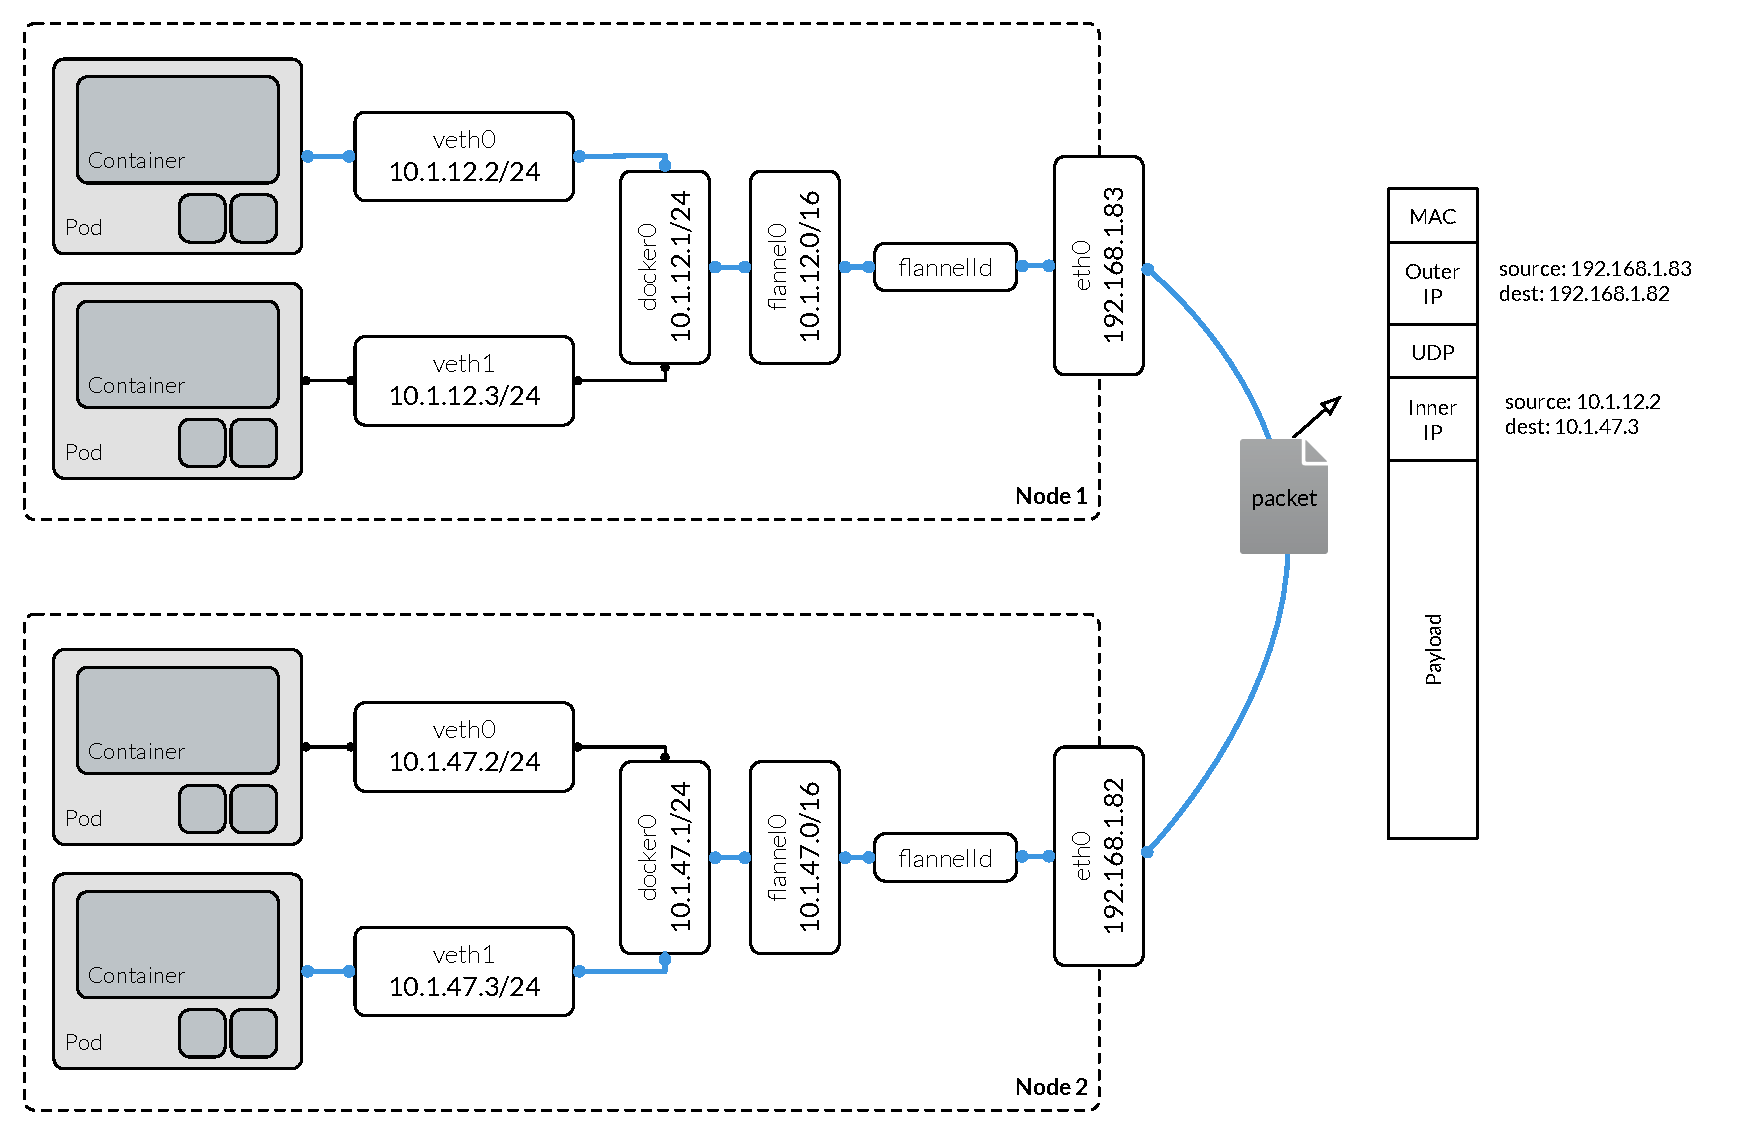
\includegraphics[width=\textwidth]{figures/kubernetes/flannel_networking}
    \caption{Flannel Networking}
    \label{fig:flannel}
\end{figure}

\noindent Figure~\ref{fig:flannel} shows two nodes in a Kubernetes cluster. Each node has the Docker engine and a flannel agent running. The example shows how the pod-to-pod communication is achieved. Every pod is assigned a virtual IP provided by the docker0 subnet. The docker0 subnet is controlled and assigned by flannel. Flannel stores these configurations in etcd, which makes it possible to map between host IP and virtual IP. As seen from the payload, Node 1's packet contains an inner IP destination with the virtual IP of the pod and an outer IP destination with the host machine's IP (Node 2). This mapping helps decouple pod and machine, and multiple pods on the same machine can expose the same port.